% !TeX spellcheck = en_GB
\section{More on Fractals}
Here will be discussed some extensions of famous fractals studied before (in \ref{fractalsExamples}).
This is not directly relevant for this paper, but an involved reader may be interested.

\subsection{Mandelbrot and Julia Sets}
%plots represent numbe of iterations and blah


\subsection{Sierpiński Fractals}
Following the idea of Sierpiński carpet, several othe fractals may be generated.
First, using (equilateral) triangles instead of squares:

\begin{wrapfigure}{r}{5cm}
	\vspace{-0.5cm}
	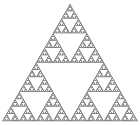
\includegraphics[width=6cm]{SierpinskiTriangle}
	\centering
	\captionsetup{justification=centering}
	\caption{Sierpinski Triangle (8 steps)}
	\label{fig:SierpinskiTriangle}
	\vspace{-3cm}
\end{wrapfigure}
\subparagraph{Sierpiński Triangle}
Sierpiński triangle is also a fractal constructed recursively by removing parts of its initial set, following a pattern similar to the one for Sierpiński carpet (although, there are equivalent definitions).

The construction is starts from an equilateral triangle.
Then, at each step, split every equilateral triangle into 4 sub-triangles as follows:\\
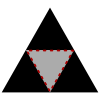
\includegraphics[width=4cm]{SierpinskiTriangleStep}\\
Remove the central triangle, and repeat the operation on the remaining 3 triangles.

The figure is made of $3$ copies of itself, scaled by a factor of $\frac{1}{2}$.
Therefore, the intuitive Hausdorff dimension for this set is $\dim_H(K) = \frac{log(3)}{log(2)} \approx 1.585$.
Again, this can be proved rigorously using similar techniques as in \cite[p. 34-35, ex. 2.7]{Falconer_1990}.

\paragraph{Sierpiński 3D Fractals}
Seen previously, Sierpiński carpet and triangle live in a 2D world, but the idea of Sierpiński fractal may also be extended to 3D.

\begin{wrapfigure}{r}{5.75cm}
	\includegraphics[width=6cm]{MengerSponge}
	\centering
	\captionsetup{justification=centering}
	\caption{Menger Sponge \\(4 steps)}
	\label{fig:MengerSponge}
	\vspace{-0.5cm}
\end{wrapfigure}
\subparagraph{Menger sponge}
The Menger sponge is the generalisation of Sierpiński carpet to 3 dimensions.

Start with a cube; split it into 27 identical copies scaled by $\frac{1}{3}$, and remove the central one, and the 6 cubes sharing a face with the central cube.
Repeat this operation on each of the 20 remaining cubes.

From this construction arise a fractal with dimension $\frac{log(20)}{log(3)} \approx 2.727$.

\begin{wrapfigure}{r}{5cm}
	\vspace{-0.5cm}
	\includegraphics[width=5.25cm]{SierpinskiTetrahedron}
	\centering
	\captionsetup{justification=centering}
	\caption{Sierpiński Tetrahedron \\(5 steps)}
	\label{fig:SierpinskiTetrahedron}
	\vspace{-1.25cm}
\end{wrapfigure}
\subparagraph{Sierpiński tetrahedron}
The Sierpiński tetrahedron (or tetrix) is the analogue of Sierpiński triangle in 3 dimensions.
Start with a regular tetrahedron; split it into 5 identical copies scaled by $\frac{1}{2}$, and remove the central one.
Repeat this operation on each of the 4 remaining tetrahedrons.

From this construction arise a fractal with dimension $\frac{log(4)}{log(2)} = 2$.
Note that this set is dimension exactly 2 while not being a surface.

\subsection{Coastline of Islands}\label{appendix:coastlines}
The coastline can be measured at different scales.
As the scale is refined, one measures a more detailed curve, which leads to a larger length.
This refinement can be done indefinitely: from segments of $1000km$ (one would only capture the rough coastline shape) to segments of $1mm$ (one would need to go around every grain of sand), and even further considering sub-atomic scales.

Following this reasoning, the (1D) length of coastlines is infinite.
It is in fact a fractal with dimension greater than one (but less than 2, as contain in a plane).

It is then possible to measure how disordered the coastline of an island is, by approximating its Hausdorff dimension.
This will be done macroscopically, using maps extracted from the Google Maps service.
In this paper, 3 islands will be considered: The United Kingdom, Iceland, and Madagascar.
The United Kingdom and Iceland are understood as having messy coastlines (so should have a high Hausdorff dimension), whereas Madagascar is though to have a rather smooth coastline (Hausdorff dimension close to one).

\begin{figure}[!h]
	\includegraphics[scale=0.6]{UKCoastlines}
	\hspace{1.5cm}
	\includegraphics[scale=0.5]{IcelandCoastlines}
	\hspace{1.5cm}
	\includegraphics[scale=0.55]{MadagascarCoastlines}
	\centering
	\caption{Coastlines (coloured in green) of the UK, Iceland, and Madagascar.}
	\label{fig:islandsCoastlines}
\end{figure}

Of course, fractal dimension can only be an approximation.
We approach the problem as follows:
First, we take a high resolution map of the island, and split it into a binary colour image, black for the ground, and white for the surrounding sea (as in fig. \ref{fig:islandsCoastlines}).
Then, we reduce the size of the image by merging pixels ("pixelizing") to obtain lower resolution images.
The resolution panel will correspond to the measuring scales panel.
A subset of the resulting images is shown in fig. \ref{fig:islandsScales}.

\begin{figure}[!h]
	\includegraphics[width=15cm]{UKScales}\\
	\includegraphics[width=15cm]{IcelandScales}\\
	\includegraphics[width=15cm]{MadagascarScales}
	\centering
	\caption{Map scales for the UK, Iceland, and Madagascar.}
	\label{fig:islandsScales}
\end{figure}

Now, using computer vision (as a Python package), we obtain the contours of the shape in an image.
It is then straightforward to measure the length of the contour (in pixels, which can be converted to kilometres as we know the scale of the image).
Repeating this operation for each scale of the map gives an array of coastline length with associated scales.

Plotting the values in a log-log plot show a nearly straight line; the approximate dimension will be given by the slope of the best fitting line.
We obtained the following dimensions:

\begin{tabular}{l l}\label{table:islandsDimensionRegression}
	\textbf{United Kingdom} & $D \approx 1.2354$ \\
	\textbf{Iceland}        & $D \approx 1.2466$ \\
	\textbf{Madagascar}     & $D \approx 1.0600$
\end{tabular}

The fitting line is very close to the data (see fig. \ref{fig:islandsDimensionRegression}), showing that the behaviour is as expected.

\begin{figure}[!h]
	\includegraphics[width=5.25cm]{UKDimensionRegression}
	\hspace{0.25cm}
	\includegraphics[width=5.25cm]{IcelandDimensionRegression}
	\hspace{0.25cm}
	\includegraphics[width=5.25cm]{MadagascarDimensionRegression}
	\centering
	\caption{Islands Dimension Regression}
	\label{fig:islandsDimensionRegression}
\end{figure}

The full code for this study can be found here: \url{https://colab.research.google.com/drive/1qo8S8oxqcLsw9UFrq5wTuVyxVA48uwFF?usp=sharing}.

